%! TEX program = xelatex
% \documentclass[draft]{beamer}
\documentclass[compress]{beamer}

\usepackage{kotex}
\usepackage{minted}

\usepackage{tikz}
\usetikzlibrary{patterns,decorations.pathmorphing}

\usepackage[export]{adjustbox}

\vfuzz=30pt
\hfuzz=5pt

%%%%%%%%%%%%%%%%%%%%%
%  Beamer Settings  %
%%%%%%%%%%%%%%%%%%%%%
\usetheme[numbering=fraction,subsectionpage=progressbar]{metropolis}
\usecolortheme{rose}
\useoutertheme[subsection=false]{miniframes}

\setbeamertemplate{itemize item}[square]
\setbeamertemplate{itemize subitem}[triangle]
\setbeamertemplate{itemize subsubitem}[circle]

% \usepackage{pgfpages}
% \setbeameroption{show notes on second screen}

% A workaround to make miniframes circles clickable with XeTeX
% See https://tex.stackexchange.com/a/369327
\setbeamertemplate{mini frame in current section}{%
  \visible<0>{\resizebox{0.1cm}{0.1cm}{o}}\kern-0.1cm%
  \begin{pgfpicture}{0pt}{0pt}{0.1cm}{0.1cm}
    \pgfpathcircle{\pgfpoint{0.05cm}{0.05cm}}{0.05cm}
    \pgfusepath{stroke}
  \end{pgfpicture}%
}
\setbeamertemplate{mini frame in current subsection}{%
  \visible<0>{\resizebox{0.1cm}{0.1cm}{o}}\kern-0.1cm%
  \begin{pgfpicture}{0pt}{0pt}{0.1cm}{0.1cm}
    \pgfpathcircle{\pgfpoint{0.05cm}{0.05cm}}{0.05cm}
    \pgfusepath{stroke}
  \end{pgfpicture}%
}

% Set footline
% See https://tex.stackexchange.com/a/386633
% \setbeamercolor{section in head/foot}{fg=normal text.bg, bg=structure.fg}
% \setbeamercolor{subsection in head/foot}{fg=normal text.bg, bg=structure.fg}
% \makeatletter
% \setbeamertemplate{footline}{%
%     \begin{beamercolorbox}[colsep=1.5pt]{upper separation line head}
%     \end{beamercolorbox}
%     \begin{beamercolorbox}{section in head/foot}
%       \insertsubsectionnavigationhorizontal{\paperwidth}{}{\hskip0pt plus1filll}\vskip3pt%
%     \end{beamercolorbox}%
%     \begin{beamercolorbox}[colsep=1.5pt]{lower separation line head}
%     \end{beamercolorbox}
% }
% \makeatother

%%%%%%%%%%%%%%%%%%%
%  Font Settings  %
%%%%%%%%%%%%%%%%%%%
\usepackage[factor=500]{microtype}

\usefonttheme{professionalfonts} % required for mathspec
\usepackage{mathspec}

\setmathsfont(Digits)[%
  Numbers={Lining, Proportional}
]{Fira Sans}
\setsansfont[%
  BoldFont={Fira Sans SemiBold},
  Numbers={OldStyle}
]{Fira Sans}
\setsanshangulfont{Noto Sans CJK KR}[%
  AutoFakeSlant=0.18,
  FontFace={m}{up}{Font=*}
]

\newfontfamily\NotoSansMonoExtraCondensed{Noto Sans Mono ExtraCondensed}
\RenewDocumentCommand\UrlFont{}{\NotoSansMonoExtraCondensed}
\NewDocumentCommand\textct{m}{{\NotoSansMonoExtraCondensed#1}}

\usepackage{contour}
\contourlength{1pt}

%%%%%%%%%%%%%%%%%%%%%
%  Minted Settings  %
%%%%%%%%%%%%%%%%%%%%%
\renewcommand\theFancyVerbLine{\textsf{\tiny\arabic{FancyVerbLine}}}
\newminted{latex}{
  escapeinside=||,
  autogobble,
  linenos,
  breaklines,
  numbersep=5pt,
  frame=single,
  fontsize=\footnotesize}
\newmintinline[ltxverb]{latex}{}
\NewDocumentCommand\inputltx{m}{%
  \inputminted[
    escapeinside=||,
    autogobble,
    linenos,
    breaklines,
    numbersep=5pt,
    frame=single,
    fontsize=\footnotesize
  ]{latex}{#1}}


%%%%%%%%%%%%%%%%%%%%%%%
% Custom Settings  %
%%%%%%%%%%%%%%%%%%%%%%%
\NewDocumentCommand\beamer{}{\textsc{beamer}}
\NewDocumentCommand\tpc{}{\!\textperiodcentered\!}
\NewDocumentCommand\tat{}{\textasciitilde}
\NewDocumentCommand\tla{}{\textleftarrow}
\NewDocumentCommand\tra{}{\textrightarrow}
\NewDocumentCommand\tua{}{\textuparrow}
\NewDocumentCommand\tda{}{\textdownarrow}
\NewDocumentCommand\tbs{}{\textbackslash}
\NewDocumentCommand\vpad{}{\vspace{1em}}

\newcommand*{\numberofpages}[1]{%
  \the\XeTeXpdfpagecount"#1"%
}

%%%%%%%%%%%%%%%%%%%%%%%
%  Document Settings  %
%%%%%%%%%%%%%%%%%%%%%%%
\title{\textsc{beamer}}
\subtitle{내용 중심의 프레젠테이션}
\author{이재호}
\institute{서울대학교 전기\tpc{}정보공학부\,/\,KTUG}
\date{2020년 5월 30일}

%%%%%%%%%%%%%%
%  Document  %
%%%%%%%%%%%%%%
\begin{document}
% \RenewDocumentCommand\pause{o}{}

\maketitle

% Hook
\begin{frame}
  \setbeamercovered{transparent}
  \Large\centering\onslide<1>{Impressive}\onslide<2->{ vs Informative}\\
  \vpad\large
  \only<-2>{PowerPoint나 Keynote, Prezi의 현란한 화면 전환 효과}
  \only<3>{청중에게 전달하고자 하는 핵심을 담은 내용}
  \pause\vpad

  \setbeamercovered{invisible}
  \only<2>{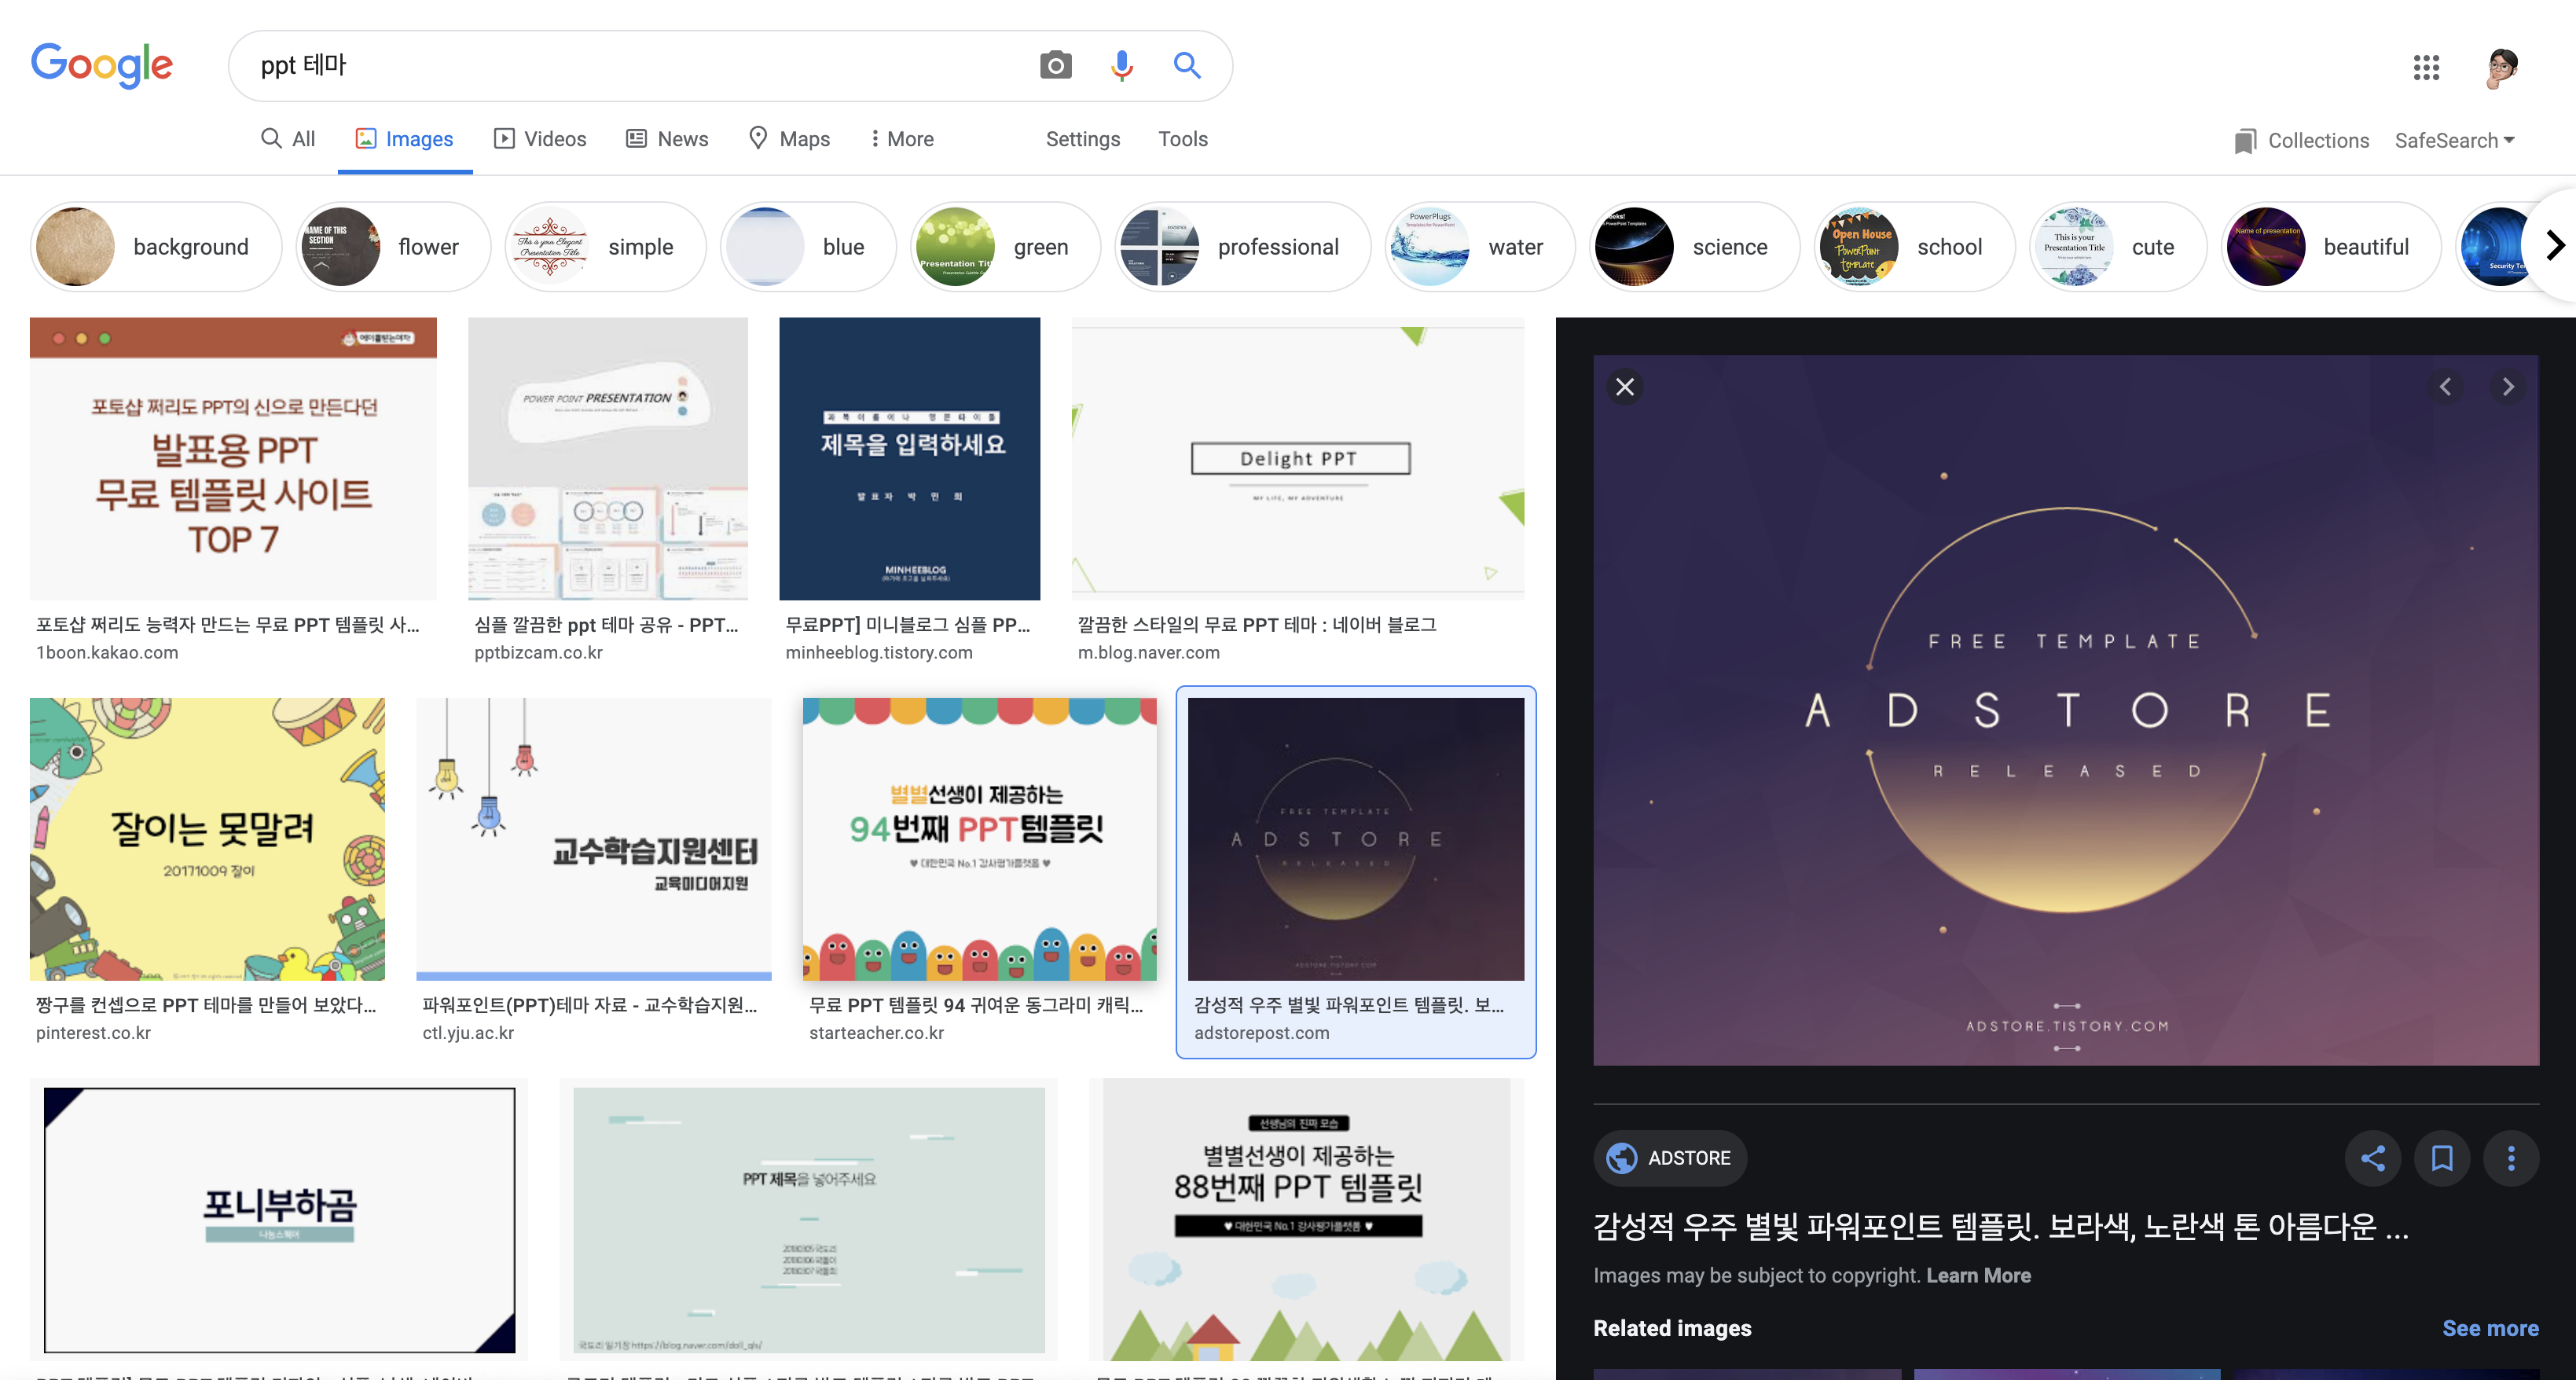
\includegraphics[width=0.85\textwidth]{figures/ppt-themes.png}}
  \begin{onlyenv}<3>
    \begin{tikzpicture}
      \begin{scope}[blend group = soft light]
        \fill[red!23!white] (0:1.2) circle (2);
        \fill[blue!23!white] (180:1.2) circle (2);
      \end{scope}
      \node[font=\small] at (0:2) {%
        \begin{tabular}{c}내용 중심의\\프레젠테이션\end{tabular}};
      \node[font=\Large] at (180:2) {\LaTeX};
      \node{\beamer};
    \end{tikzpicture}%
  \end{onlyenv}

  \note{
    프레젠테이션은 두 가지 방식으로 만들 수 있다.
    항상 상호배타적인 것은 아니지만, impressive할 것인가, 아니면 informative할
    것인가.
    내용이 부실하더라도 예쁜 색상과 스타일리시한 테마, 화려한 효과로 꾸밀 수
    있다.
    발표 자료를 공들여 만들어보신 적이 있다면, 분명히 검색 엔진에서 ``ppt
    테마''라고 검색해보셨을 것이다.
    PowerPoint를 쓸지, Prezi를 쓸지, macOS를 쓰는 분이라면 Keynote를 쓸지
    고민도 하셨을 것이다.
    다만, 이 모두는 사실 부수적인 ``디테일''에 불과하다.
    정작 발표하려는 내용에 투자할 시간을 뺏길 수 있다.
    오히려, 덜 전문적으로 보일 수도 있다.

    \TeX을 아시고 쓰시는 여러분은, 수식, 코드, 다이어그램을 사용하여
    발표할 일이 많으실 것이라고 생각된다.
    자연스레, ``\LaTeX을 사용해서 발표자료를 만들 수 있을까?''라는 고민을 할
    것이다. (저만 그런가요?)
    \LaTeX을 사용해서, 내용 중심의 프레젠테이션을 할 수 있는 도구가 바로
    \beamer이다.

    이 자리에서는 \beamer를 사용해서 어떻게 발표 자료를 만들 수 있을지
    소개해드리려고 한다.
  }
\end{frame}

\begin{frame}{목차}
  \tableofcontents
\end{frame}

\section{도입}
\subsection{\textsc{beamer}에 대하여}
\begin{frame}[fragile]{\textsc{beamer}의 장점}
  \begin{itemize}
    \item \alert{\LaTeX을 사용할 수 있음}\pause
      \begin{itemize}
        \item 수식: $\nabla \cdot \vec E = \frac{\rho}{\varepsilon_0}$\pause
        \item 코드: \ltxverb/Hello, \LaTeX!/\pause
        \item 도식 (TikZ):\\
          %%%%%%%%%%%%%%%%%%%% sample TikZ code
          \begin{tikzpicture}
            \tiny
            % surface
            \draw (-0.2, 1.2) -- (0.75, 0.25) .. controls (1, 0) ..  (1.25, 0)
              -- (4, 0) -- (4, 0.4);
            \draw[dashed] (-0.2, 0) -- (1.25, 0);
            % label
            \draw[latex-latex] (0.09, 0.91) -- node[anchor=east] {$h$} (0.09, 0);
            \draw[latex-latex] (2.75, 0.3)
              -- node[anchor=south] {$2L$} (3.55, 0.3);
            % boxes
            \draw[fill=gray, rotate around={45:(0, 1)}] (0, 1) rectangle
              node {\contour*{white}{$m$}} (0.25, 0.75);
            \draw[fill=gray, opacity=0.5] (2.5, 0) rectangle (2.75, 0.25);
            \draw[fill=gray, opacity=0.5] (3.3, 0) rectangle (3.55, 0.25);
            % springs
            \draw[densely dotted,
              decoration={coil,amplitude=3,segment length=5,aspect=0.5},
              decorate] (2.75, 0.125) -- (4, 0.125);
            \draw[decoration={coil,amplitude=3,segment length=1,aspect=0.5},
              decorate] (3.55, 0.125) -- (4, 0.125);
            \node[anchor=south east, yshift=3] at (4, 0.125) {$k$};
          \end{tikzpicture}
          %%%%%%%%%%%%%%%%%%%%
      \end{itemize}
      \pause

    \item 자동화 (목차 생성, 반복문, \ldots)\pause
      \begin{itemize}
        \item expl3을 활용한 코딩
          \footnotesize
          \ltxverb/\int_step_inline:nn{4}{\int_step_inline:nn{#1}{*}\\}/:
          \scriptsize\ExplSyntaxOn
          \int_step_inline:nn{4}{\int_step_inline:nn{#1}{*}\\}
          \ExplSyntaxOff
      \end{itemize}
      \pause

    \item \alert{구조화된 문서}
  \end{itemize}
\end{frame}

\begin{frame}{\textsc{beamer}의 또다른 장점}
  \begin{itemize}
    \item 한 번 만든 템플릿을 쉽게 재활용
    \item PDF 문서로 만들어지므로 어디에서든 열어볼 수 있음
      \begin{itemize}
        \item \alert{모든 곳에서 깨지지 않고 동일한 형태로 보임}
      \end{itemize}
    \item 학술적인 용도로 굉장히 많이 사용됨
      \begin{itemize}
        \item 자료와 커뮤니티가 방대함
      \end{itemize}
    \item \alert{이미 작성한 \LaTeX{} 문서를 재활용}하여 발표 자료를 만들 수 있음
    \item 최신 \TeX{} 배포판이 깔려 있다면 따로 설치할 필요가 없음
  \end{itemize}
\end{frame}

\subsection{템플릿}
\begin{frame}{템플릿 찾기}
  \beamer를 가장 쉽고 빠르게 사용하고 배우는 방법은 미리 만들어진 템플릿을
  사용하는 것

  \begin{block}{유용한 자료}
    \begin{itemize}
      \item \url{http://www.texample.net/tikz/examples/tag/beamer/}
      \item \url{https://www.overleaf.com/gallery/tagged/presentation}
      \item \url{https://latex.simon04.net/}
      \item \url{https://users.cs.northwestern.edu/~jesse/code/beamer-examples/}
      \item \href{https://github.com/Zeta611/beamer-tutorial-latex-workshop-2020}{본 발표 자료}
    \end{itemize}
  \end{block}
\end{frame}

\begin{frame}[fragile]{템플릿에서 바꿀 내용}
  \begin{alertblock}{바꿀 명령어}
    \begin{itemize}
      \item \ltxverb/\title[short]{long}/
      \item \ltxverb/\subtitle[short]{long}/
      \item \ltxverb/\author[short]{long}/
      \item \ltxverb/\date[short]{long}/
      \item \ltxverb/\institute[short]{long}/
    \end{itemize}
  \end{alertblock}
  \verb/short/, \verb/long/은 각각 각주 등에 표시될 짧은 표기와 표지에 표시될
  정식 표기를 말한다.
\end{frame}

\subsection{\texttt{frame}}
\begin{frame}[fragile]{Hello, \textsc{beamer}!}
  \begin{block}{\texttt{hello-beamer-1.tex}}
    \begin{columns}
      \begin{column}{0.5\textwidth}
        \small
        \inputltx{tutorial/hello-beamer-1.tex}
      \end{column}
      \begin{column}{0.4\textwidth}
        \ExplSyntaxOn
        \int_set:Nn \l_tmpa_int { \numberofpages{tutorial/hello-beamer-1.pdf} }
        \begin{overprint}
          \int_step_inline:nn { \l_tmpa_int }
            {
              \onslide<#1>
              \includegraphics[
                frame, page=\int_eval:n { #1 }, width=\textwidth
              ]{tutorial/hello-beamer-1.pdf}\\
            }
        \end{overprint}
        \ExplSyntaxOff
      \end{column}
    \end{columns}
  \end{block}
\end{frame}

\begin{frame}[fragile=singleslide]{\texttt{frame}}
  \begin{columns}
    \begin{column}{0.5\textwidth}
      \begin{latexcode}
        \begin{frame}[c]
          \frametitle{Foo}
          Bar
        \end{frame}
      \end{latexcode}
    \end{column}
    \begin{column}{0.5\textwidth}
      와 다음은 같다:
      \begin{latexcode}
        \begin{frame}[c]{Foo}
          Bar
        \end{frame}
      \end{latexcode}
    \end{column}
  \end{columns}
  \vpad
  \begin{alertblock}{\texttt{frame}의 정렬}
    기본적으로 정렬은 \verb/[c]/로 가운데 정렬이며, 이외에 \verb/[t]/
    (위 정렬)와 \verb/[b]/ (아래 정렬)가 있다.
  \end{alertblock}
\end{frame}

\section{내용 넣기}
\subsection{리스트}
\begin{frame}[fragile=singleslide]{\texttt{itemize}}
  \begin{block}{\texttt{hello-beamer-2.tex}}
    \begin{columns}
      \begin{column}{0.5\textwidth}
        \begin{latexcode}
          \begin{frame}
            \frametitle{First Slide}
            \begin{itemize}
              \item TikZ
              \item Beamer
                \begin{itemize}
                  \item Fun
                  \item Cool
                  \item Sexy
                \end{itemize}
            \end{itemize}
          \end{frame}
        \end{latexcode}
      \end{column}
      \begin{column}{0.4\textwidth}
        \includegraphics[
          frame,page=2,width=\textwidth
        ]{tutorial/hello-beamer-2.pdf}
      \end{column}
    \end{columns}
  \end{block}
\end{frame}

\begin{frame}[fragile=singleslide]{글머리 기호 바꾸기}
  기본값인 \verb/default/ (\verb/triangle/), 원형 \verb/circle/, 사각형
  \verb/square/, 그리고 구형 \verb/ball/ 중에서 고를 수 있다.
  \vpad
  \begin{exampleblock}{예시}
    \begin{latexcode}
      \setbeamertemplate{itemize item}[ball]
      \setbeamertemplate{itemize subitem}[square]
      \setbeamertemplate{itemize subsubitem}[triangle]
    \end{latexcode}
    \setbeamertemplate{itemize item}[ball]
    \setbeamertemplate{itemize subitem}[square]
    \setbeamertemplate{itemize subsubitem}[triangle]
    \begin{itemize}
      \item 실수
        \begin{itemize}
          \item 정수
            \begin{itemize}
              \item 자연수
            \end{itemize}
        \end{itemize}
    \end{itemize}
  \end{exampleblock}
\end{frame}

\begin{frame}[fragile=singleslide]{\texttt{enumerate}와 \texttt{description}}
  \begin{block}{\texttt{hello-beamer-3.tex}}
    \begin{columns}
      \begin{column}{0.5\textwidth}
        \begin{latexcode}
          \begin{frame}{Second Slide}
            \begin{enumerate}
              \item item1
              \item item2
            \end{enumerate}
            \begin{enumerate}[(a)]
              \item item1
              \item item2
            \end{enumerate}
            \begin{description}
              \item[key] value
              \item[long key] value
            \end{description}
          \end{frame}
        \end{latexcode}
      \end{column}
      \begin{column}{0.4\textwidth}
        \includegraphics[
          frame,page=3,width=\textwidth
        ]{tutorial/hello-beamer-3.pdf}
      \end{column}
    \end{columns}
  \end{block}
\end{frame}
\end{document}
